
\chapter{Solution Development}\label{chapter:analysis}
In a previous work on this topic, Wörndl and Herzog  \parencite{cbrecsys2014} drew inspiration for their formal model based on the Oregon Trail knapsack problem (see Section \ref{sec:oregon}); they formulated a model that extends the value function of the problem using a penalty function.

For clarity, we adjusted the notation used in their paper to fit the notations used in previous function values. Wörndl and Herzog formally defined their value function as follows:

\begin{gather}
 \tag{1} f_j(x_j, x_{d_j}) = x_j \cdot v_j - \sum_{e \in x_{d_j}} ( t(j, e) \cdot x_j \cdot v_j \cdot [x_e > 0])\label{eq:3d}
\end{gather}

where $v_j$ is the value of region $j$ (i.e, item) for the specified user query, and $t(j, e)$ is the penalty function for the two regions $j$ and $e$. Their value function is similar to the function Type \ref{eq:2g} specified by the original Oregon Trail knapsack model. However, the previously defined value-reducing constant factor $t$, is a function of the two regions $j$ and $e$. 

Wörndl and Herzog’s formal model is defined as follows:
\begin{align}
    \tag{1}maximize \qquad  &\sum_{i=1}^n  f_j(x_j, x_{d_j}) \label{eq:3a}\\
    \tag{2}subject \ to \qquad &\sum_{i=1}^n x_i d_i  \leq D \label{eq:3b}\\
    \tag{3}&\sum_{i=1}^n x_i\ b_i \leq B \label{eq:3c}\\
    \tag{4} &x_i \in \{0,1\}
\end{align}

where $f_j(x_j, x_{d_j})$ is the penalty function defined in \ref{eq:3d}; $d_i$ is item $i$'s recommended duration of stay, and $b_i$ is item $i$'s recommended daily budget. $D$ is the maximum possible duration of stay and $B$ is the maximum budget the user can spend on their trip. 

Wörndl and Herzog concluded that the penalty function defined in their work could be improved to produce better results. Building penalty-based functions requires careful consideration of the function parameters and the function itself. Thus, to gain freedom from the influence of the penalty function, we reformulate and extend the problem definition to a non-penalty-based approach. If through further analysis, a penalty-based approach proves to be a better fit for our selected algorithm, we will redefine a penalty function as needed.

The framework for our \gls{rs} comprises a knapsack model for the multi-objective \gls{op}, a data model, and a meta-heuristic solution. In the following sections, we analyze these three parts in detail.


\section{Problem Reformulation} \label{sec:problem_definition}

Let us consider $n$ regions $(i = 1, ..., n)$. Each region $i$ will have $k$ profits $s_{ik}\ (p = 1, ...,k)$. Given a set $N$ of $m$ traveling preferences $N = \{N_1, N_2,...,N_m\}$, $s_{ik}$ is dependent on $i$'s score on $N$. For example, a region can have a different score for shopping and another for hiking.
The recommendation problem can be modeled as a multi-objective \gls{op}. Given a user query, some regions must be selected to maximize the $p$ total profits while not exceeding the budget limit $B$ and the total stay duration $D$. Each user preference must be fulfilled by at least one of the selected regions. Assuming the system recommends Trip $T$ comprising $n$ regions ($T = {x_1, x_2, ..., x_n}$), the physical distance between a region $x_i$ and its neighbor $x_2$ should not exceed a defined constant $\sigma$. In a case in which no location coordinates for the regions are available, the regions in the recommended trip should be within reasonable distance from one other. Additionally, the duration of stay in a particular region ${x_i}$ should ensure a minimum utility value, which is defined in the algorithm.

The mathematical model of the \gls{moop} is defined as follows:

\begin{align}
    \tag{1}maximize \qquad  &z_n(x) = \sum_{k=1}^p x_i\ s_{ik}, \hspace{1cm} i = 1,...,n \label{eq:3_1a}\\
    \tag{2}subject \ to \qquad &\sum_{i=1}^n x_i\ d_i  \leq D \label{eq:3_1b}\\
    \tag{3}&\sum_{i=1}^n x_i\ b_i \leq B \label{eq:3_1c}\\
    \tag{4}&\sum_{j \in N} x_{ij} \geq 1 \label{eq:3_1e}\\ 
    \tag{5}&\sum_{i=1}^n x_{i} \ g(p_i) \leq \sigma,  \hspace{1cm}  \label{eq:3_1f} \\
    \tag{7} x_i \in \{0,1\}, \qquad &\forall \ 1 \leq i \leq n \label{eq:3_1f2}
\end{align}

where $x_i = 1$ when item $i$ is chosen; otherwise $x_i = 0$. 
Constraints \ref{eq:3_1b} and \ref{eq:3_1c} represent the constraints on total stay duration and budget, respectively. Equation \ref{eq:3_1e} ensures that each user preference is satisfied at least once. Constraint \ref{eq:3_1f} represents the physical distance between the regions, in which $g$ is a function of the physical location. It is assumed that all coefficients $s_{ik}, b_{i}, B, d_i,$ and $D$ are positive. 

\subsection*{Pareto Optimum}
There are multiple scores to be maximized in the objective function. Therefore, choosing an objective maximizing optimal solution without trade-offs is infeasible. In multi-objective optimization, Solution $s$ is said to dominate $s'$ if $s$ is at least as good as $s'$ in every criterion, and $s$ is better in at least one criterion; $s \succ s'$ is used to denote such a case. If no solution dominates Solution $s^*$, then $s^*$ is said to be \textit{Pareto optimal} (i.e., non-dominated). The set of all non-dominated vectors is known as the \textit{Pareto front}.

\textbf{Example}:
Figure \ref{fig:moopsample} a two-objective instance of the \gls{moop} problem. For simplicity, we assume two given preferences. The gray box displays the user input. When mapped to our problem definition, there are two objectives to be maximized, where an objective represents a single item. An item can be any \gls{poi}, for example attraction sites, region, or route. $f = (\Vec{f_1}, \Vec{f_2}, ... ,\Vec{f_k})$ represents all feasible solutions. We compute a solution in the objective space $\Vec{f_i} = (z_1, z_2)$. The objective values are computed on preferences $M$ and $S$, while respecting the necessary constraints. Parameter $x$ in the illustration is a boolean array that encodes the selection of an item combination. The selected item combinations are subject to the notion of Pareto optimality defined above. For example $f_7 \succ f_2$ because it is better in at least one of its objective values as $f_2$ and it is strictly better in another value. The Pareto front consists of the selections $\{f_1,f_5,f_7,f_9,f_{10}\}$, and we achieve a total score of (24, 23). 


\begin{figure}[ht!]
    \centering
    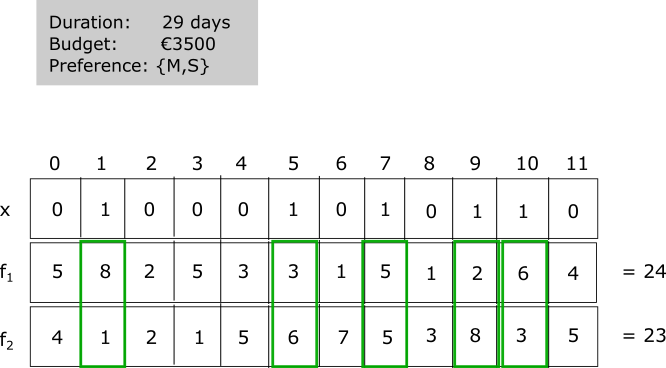
\includegraphics[width=8cm]{Moop}
    \caption{Example solution to the multi-objective orienteering problem}
    \label{fig:moopsample}
\end{figure}

Pareto optimality here implies that there is no item combination $f_k$ that will improve the achievable score of at least one item without diminishing the achievable score of another item.

We can also extend the concept of Pareto optimality from the solution space to the objective space. Given $n$ objective functions $z = (z_1,...,z_n)$, with each objective having a score $\Vec{v} = (v_1,...,v_j)$ on $j$ criteria, we define the concept of Pareto optimality in the objective space as follows. An objective $z$ dominates an objective $z'$, denoted by $z \succ z'$, if
\begin{itemize}
    \item $z_i(v) \geq z_i'(v)$ on each score of $\Vec{v_j}$; and
    \item there exists one score $v^*$ such that $z_i'(v^*) > z_i'(v)$.
\end{itemize}

Again, Pareto optimality implies that there is no feasible objective $z_i$ such that $v'$ does not make it less effective in at least one other criterion.\newline
Having gained a better understanding of what is deemed optimal, an algorithm that can efficiently compute the Pareto front from a set of given items is what we aim to develop in subsequent sections.



\section{Data Model}
The underlying data model for this thesis is a travel database curated by Wörndl and Herzog \parencite{cbrecsys2014} in their previous work. The travel database contains realistic data on a region. Information about each region includes:
\begin{enumerate}
    \item Minimum weekly budget for a region
    \item Minimum duration to achieve a 25\% and 75\% utility respectively. An algorithm can either implement a minimum 25\% threshold or a 75\% minimum utility from stay threshold;
    \item The score of a region for particular travel activity preferences on a five-point Likert scale;
    \item The security score of a region on a five-point Likert scale; and
    \item The monthly weather score of a region on a five-point Likert scale (i.e., recommended months).
\end{enumerate}
The data model is hierarchically structured such that a region is always a sub-region of another region. The world is the root region, followed by the continents at the second level. Regions are geographical areas. A region could be a country, a section of a country, or a continent. For example Figure \ref{fig:datamodel} illustrates the hierarchical structure of the data model. The US and Canada are sub-regions of North America, while Alaska and Texas are sub-regions of the US. Ontario is a sub-region of Canada. The database is composed of 196 regions. All regions (except the root region) have a recommendation for a minimum stay at 25\%. Unlike previous models that calculate the connection between regions by specifying the necessary effort (time and cost) to travel from one region to another, we model connections between regions based solely on positions in the hierarchical tree structure. We extend the underlying data model to contain all sub-regions of a region. If two regions are sub-regions of the same parent, we consider them connected.

\begin{figure}
    \centering
    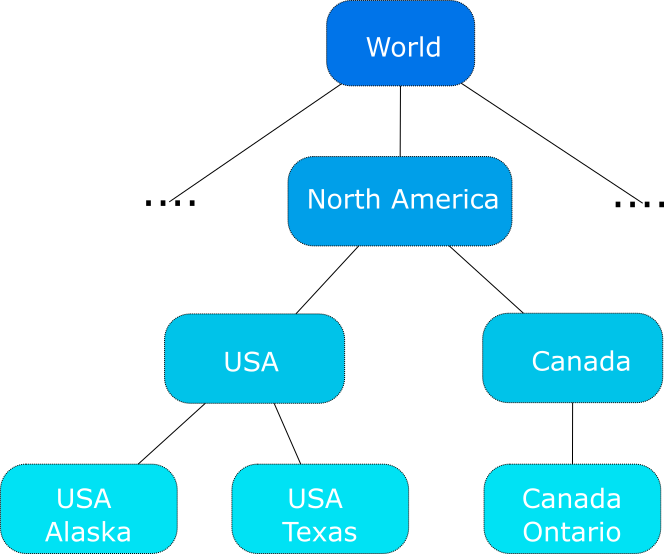
\includegraphics[width=.4\textwidth, height=.4\textwidth]{Datamodel}
    \caption{Hierarchical structure of the underlying data model}
    \label{fig:datamodel}
\end{figure}


\section{Analysis of Algorithmic Methodologies}\label{sec:alg_approaches}
According to Golden et al. \parencite{Golden1987TheProblem}, \gls{op} is an NP-hard problem. Hence, no known or expected algorithm can solve the problem optimally in polynomial time (i.e., an exact solution cannot be found within a reasonable amount of time). Computing an optimal solution with multiple objectives is even more intractable. Hence, there is usually a trade-off between time and accuracy. In multi-objective optimization, one is often interested in the Pareto front. However, it is usually infeasible to generate the exact set of a Pareto front. Reasons for this can be that the number of Pareto optima is too large, or the determination of a single Pareto optimum is computationally difficult. Therefore, the goal is usually to identify a satisfactory Pareto set approximation (i.e., a set as close to the optimum as possible \parencite{Fonseca2005AOptimizers}. Approximate algorithms offer near-optimal solutions to computationally intractable problems (mostly) in a moderate amount of time and are the major alternatives for solving NP-hard optimization problems.


Approximate algorithms can be classified as heuristics and meta-heuristics. Heuristics are usually problem dependent and inflexible (i.e., defined for a specific problem). Meta-heuristics are problem independent and can be applied to a broad range of optimization problems. In Chapter \ref{chapter:literature_review}, we found that meta-heuristic solutions are commonly used to solve \glspl{op}. Meta-heuristic solutions are also commonly used in multi-objective optimization in various research areas. Certain requirements must be considered when designing or selecting an appropriate algorithm to solve the \gls{moop}. Some requirements are intuitive for our problem domain. For example, a slow computational time by the end algorithm is intolerable for a user-oriented system. Some issues are not so intuitive. Preserving uniform diversity implies that the selected solutions in the approximated Pareto front are diverse and uniformly distributed. In addition, the \gls{moop} has been defined such that a single objective represents a single user’s preference. We are unable to pre-determine the number of preferences a user might select. A user could have just one preference. They might also have two or more preferences. Therefore, an appropriate algorithm should be applicable to a dynamic number of objectives. A brief summary of the most important requirements of the desired algorithm is as follows:
\begin{itemize}
    \item Tolerable computational time,
    \item Applicability to problem domain
    \item Uniform preservation of diversity, 
    \item Applicability to large-scale problems,
    \item Applicability to a dynamic number of objectives, and
    \item Moderate implementation complexity.
\end{itemize}



In developing an algorithm to solve our optimization problem, we first address the basic methodologies for designing an approximation algorithm. We then analyze possible heuristic and meta-heuristics solutions. In this chapter, we assume a maximization problem in which function $g$ means $f_k$ has to be maximized.

\subsection{Greedy Methods}
Greedy methods help find sub-optimal solutions that satisfy some performance guarantee in NP-hard problems. The idea is to generate a solution incrementally by making the best possible choice according to a simple criterion at each decision-making point. For example, a greedy approach to solving the simple knapsack problem is to iteratively select a node with the least weight. This approach is best used together with some form of heuristic rather than as a stand-alone method. When used alone, the heuristics generate only a minimal number of different solutions.


\subsection{Local Search}
Local search techniques range from simple heuristics to complex meta-heuristics. The basic idea behind a local search is to start from an initial (partial or non-partial) \gls{candidate solution}. The solution is improved by making local changes to it and moving from one \gls{candidate solution} to a neighboring \gls{candidate solution} until no further improvement is possible. A local change might involve removing elements from the ground set, adding elements, or swapping elements. Local search is a good heuristic for computing near-optimum solutions to reasonably sized problems. Usually, a neighborhood function $N: S \mapsto 2^S$ where $S $ is the set of feasible solutions specifies for each solution $s \in S$ a subset $N(s)$ of neighbors of $s$ (neighborhood relation), or solutions that are close to $s$ \parencite{Gonzalez2007HandbookMetaheuristics}.

For many problems, computing the locality gap (i.e., the difference between local and global optima) is complex, and the locality gap using a local natural search is commonly very large. Additionally, the algorithm might visit the exact location within the search space more than once. Thus, it can become trapped in a location far away from the global optimum. These situations all lead to very poor approximation. Consequently, many local search techniques use mechanisms to help escape a position or reduce the locality gap. For example, one could use a restart strategy when stuck in a local minimum in the iterative descent algorithm. Alternatively, one could relax the improvement criterion by performing a non-improving step. However, these strategies do not guaranty escaping an arbitrary local minimum \parencite{HolgerH2005StochasticSearch}.


\subsubsection{Iterative Improvement}
The iterative improvement algorithm is the most basic local search algorithm and forms the basis of most local search algorithms. Algorithm \ref{alg:iterative-improvement} (\textit{IterativeDescent)} produces a simple iterative improvement (also known as iterative descent). The solution of the iterative descent is the optimum local value, which may or may not be a global optimum. Condition $g(s') > g(s)$ is the evaluation of the candidate solution. solution. Evaluation functions serve as guidance to a solution \parencite{HolgerH2005StochasticSearch}. In optimization problems, the objective function’s properties usually determine the evaluation function. Below, the algorithm assumes a maximization objective function:

 \begin{algorithm}
  \caption{General outline of iterative improvement local search}\label{alg:iterative-improvement}
  \SetKwInOut{Input}{Input}
  \SetKwInOut{Output}{Output}
  \Input{Set of candidate solutions $S$, Neighborhood function $N$, Objective function $g$}
  \Output{A local optimum solution $s \in S$}
    determine an initial candidate solution $s$
    
    \While {$N(s)$ contains better solution than $s$}{
        choose a solution $s' \in N(s)$ such that\\
             \hspace{0.5cm}$g(s') > g(s)$\\
        $s := s'$\\
    }
  \end{algorithm}
  
The simple iterative improvement algorithm can be extended to multi-objective optimization problems. For multiple objectives, the solution of the iterative improvement and all local search-based algorithms, in general, is defined as the approximate set of Pareto optimal solutions (Pareto front) found during the search process. A move improves the current solution when a newly generated candidate solution is added to the approximate Pareto front. This means that the evaluation condition of the single-objective iterative improvement algorithm changes. The Pareto local search proposed by Paquete et al. \parencite{Paquete2004ParetoStudy} adapts the notion of Pareto optimality in a simple local search. First, the algorithm randomly selects one non-visited candidate solution s and examines all neighbors of s. Second, it adds all neighbors of s that are non-dominated by the set of candidate solutions. It stops when the neighborhood of all candidate solutions has been examined \parencite{Gonzalez2007HandbookMetaheuristics}. Similar to the Pareto local search, the two-criteria local search \parencite{Angel2004ApproximatingProblem} is another multi-objective adaptation of the single-objective iterative improvement algorithm. While the Pareto local search chooses only one candidate solution to examine its neighborhood and immediately updates the list of candidate solutions, the two-criteria local search examines the neighborhood of all candidate solutions in an iteration.



   
\subsection{Stochastic Local Search}
Many local search algorithms use randomized decisions, for example to determine initial solutions or when determining search steps. These are called stochastic local search (SLS) algorithms. The majority of algorithms for computing high-quality approximations to the Pareto optimal set are based on \gls{sls}. Typically, additional memory is used to store the best candidate solution from previous searches. If the solution is feasible, it is returned upon termination of the algorithm; the objective function is used to determine the quality of the candidate solutions. The performance of any \gls{sls} algorithm depends significantly on the underlying neighborhood relations and the size of the neighborhood. Determining the choice of a neighborhood relation to use for \gls{sls} is mostly problem specific. Insertion and swap are two widely used neighborhood relation-generating operators. \gls{sls} techniques are attractive because they allow solving problems using moderately generic and easily implementable algorithms that can also be extended with or adapted based on problem-specific knowledge \parencite{HolgerH2005StochasticSearch}. They range from simple constructive algorithms and iterative improvement algorithms to general algorithm frameworks adapted to a specific problem under consideration. Popular \gls{sls} algorithms include \gls{vnd}, \gls{sa}, \gls{ts}, \glspl{ea}, \gls{aoc}, and many others. 

\subsubsection{Randomized Iterative Improvement}
Using large neighborhoods is particularly beneficial to escape the local minima. However, there is an associated time complexity with performing search steps in a vast neighborhood. \gls{sls} algorithms try to implement the concept of large neighborhoods, but with trade-offs. A popular idea in \gls{sls} algorithms is to use large neighborhoods but reduce their size by never examining neighbors that are unlikely to yield any improvements in evaluation function value

Algorithm \ref{alg:randomized-iterative-improvement} is a \gls{sls}-based iterative improvement to Algorithm \ref{alg:iterative-improvement}. Algorithm \ref{alg:randomized-iterative-improvement} uses randomization as a diversification mechanism to improve the algorithm’s quality. The $\rho$ is a noise parameter that corresponds to the probability of performing a random step instead of an improvement step \parencite{HolgerH2005StochasticSearch}. The search can be terminated, for example, after a certain number of steps or after no improvement has been achieved in many steps. This algorithm outperforms the pure local search version of iterative descent; when it is run long enough, an optimal solution to any given problem instance can be found \parencite{HolgerH2005StochasticSearch}.

 \begin{algorithm}
  \caption{General outline of randomized iterative improvement local search}\label{alg:randomized-iterative-improvement}
  \SetKwInOut{Input}{Input}
  \SetKwInOut{Output}{Output}
  \Input{Set of candidate solutions $S$, Neighborhood function $N$, Objective function $g$}
  \Output{A local optimum solution $s \in S$}
    \While {termination condition not satisfied}{
        
        \eIf{there exists a solution $s ' \in N(s)$ with probability $\rho$}{
        choose solution $s' \in N(s)$ uniformly at random\\
        }
        {
        \eIf{there exists $g(s') > g(s)$ where $s' \in N(s)$}{
        choose solution $s'$ \\
        }{
        choose a solution $s' \in N(s)$ such that $s'$ is maximal \\
        }
        }
        
        $s := s'$\\
    }
  \end{algorithm}



\subsubsection{Variable Neighborhood Descent}
\Gls{vnd} algorithms benefit from the advantages of large neighborhoods by reducing the time consumed in the search steps. In the descent phase, standard small neighborhoods are used until a local optimum is encountered. Then, in the perturbation phase, the search process switches to a different neighborhood, which might help exit the corresponding basin of attraction and allow further search progress. Algorithm \ref{alg:vnd} highlights the general outline of a \gls{vnd}. Unlike the previously outlined algorithms, $N$ in this algorithm is a set $\{N_1,..., N_{imax}\}$ of neighborhood relations, usually ordered according to the increasing size of respective local neighborhoods. Variations of the \gls{vnd} algorithm have been widely and successfully applied in the single-objective domain in practice and are known to show optimal results. The algorithm can adapt to refinement and solution definitions in a multi-objective setting as defined in the iterative refinement algorithm in the previous section (see \parencite{Duarte2015Multi-objectiveProblems} for an example adaptation).

\begin{algorithm}
  \caption{General outline of variable neighborhood descent}\label{alg:vnd}
  \SetKwInOut{Input}{Input}
  \SetKwInOut{Output}{Output}
  \Input{Set of candidate solutions $S$, Set of neighborhood relations $N$, Objective function $g$}
  \Output{A local optimum solution $s \in S$}
    \While {$i < imax$}{
        choose the most improving $s'$ of $s \in N_i$\\
        \eIf{$g(s') > g(s)$}{
        $s := s'$\\
        $i := 1$
        }{
        $i := i + 1$
        }
    }
  \end{algorithm}

\subsubsection{Simulated Annealing}
\Gls{sa} is related to a probabilistic iterative improvement. It is based on the idea that the probability of accepting a deteriorating step should depend on the respective deterioration in evaluation function value, such that the worse a step is, the less likely it is that it will be performed \parencite{HolgerH2005StochasticSearch}.

The algorithm has a proposal mechanism in which a neighbor $s'$ is chosen at random, and the acceptance criteria are based on statistical mechanics (metropolis condition) as follows:

\begin{align*}
    \rho_{accept}(T,s,s') := \begin{cases}
                            1, &\text{if}\quad g(s') \geq g(s);\\
                            exp(\frac{g(s)-g(s')}{T}), &\text{otherwise};
                             \end{cases}
\end{align*}
$\rho_{accept}$ is the probability of accepting $s'$ and is parameterized by the temperature $T$ used to decide whether the search accepts $s'$ or stays at $s$. The condition above depicts the case where $T$ is kept constant and can be adjusted throughout the search process according to an annealing schedule. The technique for temperature adjustment used in simulated annealing helps escape the local minima. However, the results of simulated annealing are limited since it requires a cooling process that is typically slow in practice \parencite{HolgerH2005StochasticSearch}. Additional techniques such as neighborhood pruning, greedy initialization, low-temperature starts, and look-up tables for acceptance probabilities are typically used to achieve competitive results.

SA algorithms have been used for multi-objective optimization. Such adaptations require modifying the acceptance criterion.  Serafini \parencite{Serafini1994SimulatedProblems} provides guidelines to apply in computing the probability $\rho_{accept}$ as follows:

\begin{align*}
    \rho_{accept}(T,s,s') := \begin{cases}
                            1, &\text{if}\quad \Vec{f}(s') \succ \Vec{f}(s);\\
                            [0,1), &\text{if}\quad \Vec{f}(s) \succ \Vec{f}(s');\\
                            exp(\frac{g(s)-g(s')}{T}), &\text{otherwise};
                             \end{cases}
\end{align*}



\subsubsection{Tabu Search}
\Gls{ts} is a meta-heuristic based on adaptive memory and responsive exploration \parencite{Gonzalez2007HandbookMetaheuristics}. It guides a local heuristic search routine to explore the solution space beyond the local optimum. The algorithm forbids steps to recently visited search positions by preventing the local search from immediately returning to a previously visited candidate solution \parencite{HolgerH2005StochasticSearch}. This prevention step can be implemented by explicitly memorizing previously visited candidate solutions and ruling out any step that would lead back to those. In contrast to a simple descent method, \gls{ts} permits worsening steps, but the moves are selected from a modified part of the neighborhood. Hence, the neighborhood of s is not static. \gls{ts} algorithms are highly efficient and successfully used in a wide range of fields, including \gls{op}. It is, however, crucial to carefully choose a neighborhood relation and to use efficient caching and incremental updating schemes for the evaluation of candidate solutions \parencite{HolgerH2005StochasticSearch}. In \gls{ts} for multi-objective optimization, the central idea is to examine the neighborhood of a set of solutions, extract non-dominated solutions, and accept only some non-tabu solutions for inclusion in the approximate Pareto front. 

\subsection{Evolutionary Algorithms}
\Glspl{ea} are meta-heuristics whose methodologies are based on Darwin’s theory of evolution, where an individual in a population (set of candidate solutions) is referred to as a chromosome. A gene represents the individual’s properties. \glspl{ea} follow the same schema as shown in Algorithm \ref{alg:ea} \parencite{Gonzalez2007HandbookMetaheuristics} below. The basic principle behind \glspl{ea} is the survival of the fittest, where a fitness function based on the objective function, constraints, or some quality measure is used to select individuals from the population. For each generation (iteration), individuals compete to produce offspring \parencite{Engelbrecht2007ComputationalEdition}. An \gls{ea} might use a crossover operator to recombine two or more individuals to produce new individuals for the next generation. A mutation operator might also be used to alter the gene (characteristics of an individual) of a chromosome. The used reproduction operators depend on the chosen solution representation and the problem formulation. For example, one-point crossover, uniform crossover, and flip mutation are commonly used for representing binary string solutions. In contrast, binary string encoding is typically used for knapsack problems \parencite{Gonzalez2007HandbookMetaheuristics}.  

\begin{algorithm}
  \caption{General outline of evolutionary algorithms}\label{alg:ea}
  $P$ = apply $\tau$ on $G$ to generate $\mu$ individuals (the initial population);\\
    \While {termination criteria not met}{
        $P'$ = apply $\theta$ on $P$\Comment*[r]{selection}
        $P''$ = apply $\omega_r$ on $P'$; $r \in \{1,..,n operators\}$ \Comment*[r]{reproduction}
        $P$ = apply $\psi$ on $P$ and $P''$\Comment*[r]{replacement}
        
    }
  \end{algorithm}

\Glspl{ea} are popularly used across different industries, and Pareto-based \glspl{ea} are particularly suited for multi-objective optimization. Unlike traditional techniques such as \gls{ts}, \gls{sa}, and \gls{vnd}  that originally output a single local optimum, Pareto-based \glspl{ea} typically provide the whole set of Pareto optimal solutions in a single run, making them suitable for our problem domain. Examples of Pareto-based \glspl{ea} in literature include the \gls{nsga}, \gls{spea} and \gls{pma}.The performance of these algorithms relies on specifying a robust fitness function and estimating a good fitness-sharing parameter. The fitness-sharing parameter helps adjust an individual’s fitness based on the fitness of others. Furthermore, as in most population-based meta-heuristics, determining the initial population is important. If the initial population is not diverse, premature convergence might occur \parencite{Talbi2009Metaheuristics:Implementation}.

\subsection{Ant Colony Optimization}
\Gls{aoc} is a meta-heuristic that is part of swarm intelligence and inspired by ants. Artificial ants are designed to simulate the problem-solving behavior of ants in a colony. Ants coordinate their activities \textit{stigmergy}, an indirect communication form through modification of the environment. The idea behind ant algorithms is to use a form of artificial stigmergy to coordinate societies of artificial agents \parencite{Dorigo2018TheMetaheuristic}. An effective solution is found only through cooperation among many individuals in the colony. Inspired by the pheromones deposited by real ants, virtual ants are designed to modify numeric values (virtual pheromones) associated with different problem states. The sequence of pheromone values associated with problem states (pheromone trail) enables communication. Ants can also forget the pheromone trail history and focus on new promising search directions through an evaporation mechanism \parencite{Gonzalez2007HandbookMetaheuristics}. 

Solutions are created incrementally by moving through available problem states and making stochastic decisions at each step. Additionally, many improved and efficient \gls{aoc} algorithms make use of local searches to improve the probability of an ant choosing a component and consequently improve the quality of the solution constructed by the ants \parencite{Stutzle2000MAX-MINSystem}. \Gls{aoc} can be applied to any combinatorial optimization problem for which a constructive heuristic can be defined. However, the problem must be mapped to a representation that artificial ants can use to build solutions \parencite{Dorigo2018TheMetaheuristic}. Specifically, the problem must be representable as a construction graph $G_c = (C, L)$, where the set $L$ fully connects the components $C$. The ants exploit $G_c$ to search for an optimal solution. Fortunately, knapsack problems can be represented as a construction graph by representing the set of items as the set of components and fully connecting them. Therefore, \glspl{aoc} algorithms can be applied to our problem domain. Nevertheless, the pheromone trails, heuristics information, and solution construction must be carefully considered for the \gls{moop}. Strategies for using \gls{aoc} on multi-objective problems include aggregating the objective functions and using one ant colony with one pheromone structure or using a different colony for each objective function and having multiple pheromone structures \parencite{Alaya2007AntProblems}.

\subsection{Bee Colony Optimization}
\Gls{bco} is a meta-heuristic that represents a type of swarm intelligence inspired by bees. Artificial agents are created by partially simulating the real-life behavior of bees. Such behaviors include nectar exploration, mating during flight, food foraging, waggle dancing, and division of labor. Bee colony-based optimization algorithms are mainly based on food foraging, nest site search, and mating in the bee colony \parencite{Talbi2009Metaheuristics:Implementation}.


The \gls{aoc} algorithm is based on nest site search behavior and consists of alternating forward and backward passes. Every artificial bee explores the search space during the forward pass. It applies a predefined number of moves that construct and improve the solution, thus yielding a new solution. After obtaining new partial solutions, the bees return to the nest and begin the backward pass in which all the artificial bees share information about their solutions \parencite{Teodorovic2009BeeBCO}. The bee whose solution has the highest fitness score is selected to form the next bee population.


\section{Designing Algorithms for Multi-Objective Problems}
In the above sections, we define our optimization problem as a combinatorial multi-objective problem. Solving \gls{moop} implies obtaining an approximation set of Pareto optimal solutions in such a way that the set fulfills the requirements of convergence to the Pareto front and uniform diversity  \parencite{Talbi2009Metaheuristics:Implementation}. Exact methods such as branch and bound algorithms, constraint programming, and dynamic programming are used for two-criteria optimization problems. However, such methods are better suited for small-scale problems. In research, optimization problems with more than three objectives are often classified as multi-objective problems. This is due to the added difficulty of handling a higher number of objectives. Unlike many objective problems, two-objective and three-objective problems can be comprehensively visualized by graphical means, which makes it easier for decision makers to analyze and make better decisions \parencite{Deb2013AnConstraints}. Heuristics methods are needed for this problem scale, and designing heuristics for \gls{moop} requires additional concepts. The following sections summarize the concepts typically required for designing algorithms for \gls{moop}.


\subsection{Fitness Assignments}
The fitness assignment measures the quality of a solution by assigning a scalar-valued fitness to a vector objective function. This procedure can be classified into scalar approaches, criterion-based approaches, dominance-based approaches, and indicator-based approaches.

\subsubsection{Scalar Approaches}
Scalar approaches typically transform the \gls{moop} into single-objective problems. A scalar approach frequently used in designing solutions for multi-objective optimization problems consists of aggregating the objective functions into a single function using either addition, multiplication, or any combination of arithmetic operations. This approach has the advantage of simplifying the objective space such that only a single objective needs to be optimized. However, in order to avoid one function dominating another, aggregating the functions requires behavioral knowledge of each objective function \parencite{CoelloCoello1999ATechniquesc}. The most common aggregation method is the weighted sum approach, which is defined as follows:

\begin{gather*}
   \Vec{f} = \sum_{i=1}^k w_i f_i, \ \text{where}\ w_i \geq 0\ \text{and}\ \sum_{i=1}^k w_i = 1
\end{gather*}

where $w_i$ are coefficients representing the objectives’ relative importance, which is usually unknown. The algorithm designer must solve the problem for different values of $w_i$ and decide on the appropriate value for $w_i$ based on their intuition. Constant multipliers $c_i$ are often introduced to further reflect the importance of each objective. This helps normalize the vector function in approximately the exact numerical values. Other popular scalar approaches found in the survey by Carlos et al. \parencite{CoelloCoello1999ATechniquesc} use goal programming (minimize or maximize the absolute deviation from target to objectives) and $\varepsilon$-constraint methods (considering the objectives bound by some allowable levels $\epsilon_i$). However, transforming a \gls{moop} into a single-objective problem is not always feasible. Ascribing a hierarchy of importance to the objectives is a crucial step in aggregating the function. In our problem domain, the objective function already represents a user preference (i.e., each objective function is mapped to a particular user preference). Ultimately, assigning a level of importance to each objective function defeats the optimization problem’s purpose because the objectives are not comparable.

\subsubsection{Criterion-Based methods}
Criterion-based methods are commonly used in population-based meta-heuristics (e.g., \glspl{ea} and \gls{aoc}). They conduct the search process by treating the various objectives separately and assigning them fitness values. This procedure usually occurs in parallel or sequentially. For example, parallel approaches are used in \gls{aoc} (P-\gls{aoc} \parencite{Doerner2004ParetoSelection}), where one ant colony tackles an objective. Sequential approaches search sequentially in a defined preference order; the order signifies the importance of each objective function \parencite{Fishburn1974ExceptionalSurvey}.

\subsubsection{Dominance-Based approaches}
Dominance-based (or Pareto-based) approaches use dominance and Pareto optimality to guide the search process. In a single run, such approaches can generate a diverse set of Pareto optimal solutions and Pareto solutions in the concave portions of the convex hull of feasible objective space \parencite{Talbi2009Metaheuristics:Implementation}. Most Pareto approaches use \glspl{ea}. Compared to scalar methods, Pareto-based fitness assignment evaluates the quality of a solution in relation to the whole population by applying ranking methods. Ranks are scalar values obtained using dominance relation techniques. The rank assigned to a solution is considered its fitness value.

\subsection{Diversity Preservation}\label{sec:diversitypreservation}
Initial population selection and biased sampling during a search in population-based meta-heuristics are crucial for maintaining diversity. Diversity-preserving methods must be considered when designing meta-heuristics for \gls{moop}; they generally penalize solutions that have high density in their neighborhoods. According to \parencite{Emmerich2018AMethods}, diversity preservation strategies can be classified into kernel, nearest neighbor, and histogram methods.

\textit{Kernel methods} Kernel methods define the neighborhood of a solution according to a kernel function that takes the distance between solutions as an argument. The kernel function is applied to all distances. For example, fitness sharing is popularly used in \glspl{ea} as it degrades the fitness of an individual using a sharing function $sh$. The sharing function depends on a constant $\sigma$ and the sum of the distance between individuals in the population. $\sigma$ represents the non-similarity threshold. Nearest neighbor methods estimate the density of a solution while taking into account the distance between a solution and its $k^{th}$ nearest neighbor. For example, \gls{nsga}-II uses crowding distance sorting to sort solutions within a rank. A crowding distance of an individual $i$ is illustrated in Figure \ref{fig:crowdeddistance_sorting}. The crowding distance can be pictured as a cuboid on the $i$ and its two nearest neighbors (left and right). Equation \ref{eq:3.4a} shows the formula used to find the crowding distance for $i$ in an objective $f_k$ from $F$ objectives; it is defined as the circumference between a solution and its left and right neighbors.

\begin{figure}
    \centering
    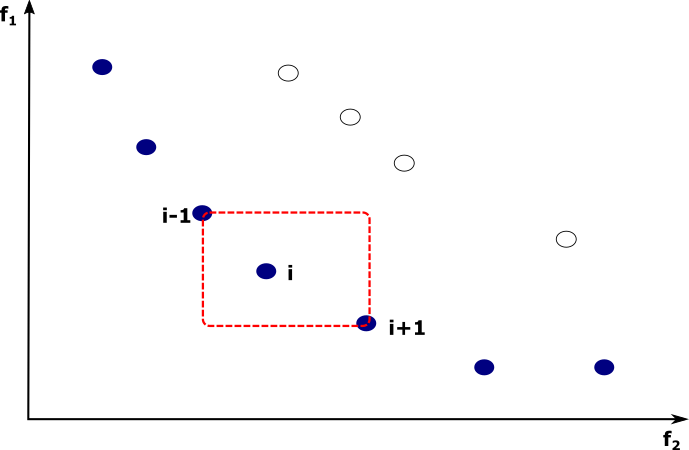
\includegraphics[width=8cm]{CrowdedDistanceSorting}
    \caption{Crowding distance sorting in \gls{nsga}-II}
    \label{fig:crowdeddistance_sorting}
\end{figure}

\begin{align}
    distance(i) = distance(i) + \frac{f_k(i+1) - f_k(i-1)}{f_k^{max} - f_k^{min}} \qquad \forall \ f_k \in F \label{eq:3.4a} 
\end{align}

More diversity is obtained using solutions with high crowding distances. Histogram-based diversity-preserving approaches partition the search space into several hyper-grids that define the neighborhood. The density around a solution is estimated by the number of solutions in the same box of a grid \parencite{Talbi2009Metaheuristics:Implementation}. The technique used to measure the distance between solutions is essential for diversity preservation. Diversity in the decision space may be essential to improve the search for some problems; however, some only require diversity in the objective space.

\section{Comparative Analysis of Choice Algorithms}
So far in this chapter, we have extensively discussed different algorithmic approaches that are commonly used to solve combinatorial optimization problems. We have presented algorithms that are typically suited for \glspl{moop}. Through our analysis, we can conclude that using traditional techniques such as local search, tabu search, etc., will be more difficult to implement for our \gls{moop} because such techniques yield a single local optimum. A single-objective optimizer needs to be run multiple times when using such techniques. Additionally, good distribution (uniform diversity) is not guaranteed. Thus, a considerable amount of adaptation is required to use these approaches for our problem domain. In contrast, modern algorithms such as the \glspl{ea}, \gls{aoc}, and \gls{bco} are best suited for multiple objective problems because they can return the Pareto optimal set in a single run. They can also be easily decomposed to find the optimal solution for single objectives. Hence, they do not require more effort than necessary to be implemented for our problem domain.

It is impossible to implement all algorithms considered suitable for our problem domain in this thesis. Thus, we compare \glspl{ea} and \gls{aoc}. These choices are based on their popularity for solving \glspl{op}, multi-objective knapsack problems, and multi-objective problems in general.

\begin{table}[htpb]
  \caption[Comparison of choice algorithms]{Comparison of choice algorithms.}\label{tab:comparison_alg}
  \centering
  \begin{tabular}{|c| c c |}
    \toprule
       &Evolutionary Algorithm &Ant-Colony \\
    \midrule
      Computational time & \checkmark &  \\ \hline
      Applicability to problem domain & \checkmark & \\\hline
      Approximate Pareto front & \checkmark & \checkmark \\\hline
      Diversity Preserving & \checkmark & \checkmark \\\hline
      Applicable to large-sized objectives & & \checkmark \\\hline
      Easier to Implement & \checkmark & \\
    \bottomrule
  \end{tabular}
\end{table}

In table \ref{tab:comparison_alg}, \glspl{ea} and \glspl{aoc} are compared using the desired algorithmic properties listed in Section \ref{sec:alg_approaches} of this chapter. The capabilities of widely used \gls{ea} variants like \gls{nsga}-II, \gls{nsga}-III, \gls{spea}2 were also taken into account. These scores are based on evaluation results from \parencite{Lust2012TheApproach, Florios2010SolvingAlgorithms, Alaya2007AntProblems}. as multi-objective knapsack problems were used for evaluation in these studies. A checkmark is awarded when the algorithm has an advantage over the other in that criterion. For example, in comparison to \glspl{aoc}, \glspl{ea} have demonstrated faster computational time in solving multi-objective knapsack problems. However, it is unknown which of the two algorithms for approximating to the Pareto front works best. \gls{aoc} is specifically designed to solve path-search problems. A graph representation of the knapsack model must be constructed, which increases the implementation complexity of the \gls{aoc}. Unlike \gls{aoc}, a number of \gls{ea} variants can be used directly for our optimization problem without adaptation. Moreover, there are several frameworks focusing on implementing \glspl{ea} that significantly decrease the time needed for implementation.\\
We can conclude that an \gls{ea} is the best algorithmic approach for our study.



 



 